\documentclass{article}

%% Original source: https://tex.stackexchange.com/questions/366229/an-aesthetically-pleasing-recipe-book-template

\usepackage{fancyhdr}
\usepackage[%
    a5paper,
%    papersize={5.5in,8.5in},
    %twoside
    margin=0.75in,
    top=0.75in,
    bottom=0.75in,
    ]{geometry}

\usepackage{xcolor}
\usepackage{wrapfig}
\usepackage{graphicx}

% Specialize colors
\definecolor{vegetarianColor}{RGB}{44, 158, 38}
\definecolor{glutenFreeColor}{RGB}{195, 124, 47}
\definecolor{drinkColor}{RGB}{48, 94, 135}
\definecolor{dessertColor}{RGB}{194, 102, 169}
\definecolor{meatColor}{RGB}{164, 10, 10}
\definecolor{fishColor}{RGB}{209, 187, 63}
\definecolor{HBRS}{RGB}{0, 157, 224}

% Change header line
\let\oldheadrule\headrule
\renewcommand{\headrule}{\color{HBRS}\oldheadrule}
\renewcommand{\headrulewidth}{2pt}%

% Headers to the page - dish type, additional dish type, serves how many
\newcommand{\dishType}[1]{\rhead{#1}}
\newcommand{\dishOther}[1]{\lhead{#1}}
\newcommand{\serves}[2][Serves]{\chead{#1 #2}}

% Dish types
\newcommand{\vegetarian}{ {\large\color{vegetarianColor}\textbf{Vegetarian}} }
\newcommand{\vegan}{ {\large\color{vegetarianColor}\textbf{Vegan}} }
\newcommand{\glutenFree}{ {\large\color{glutenFreeColor}\textbf{Gluten Free}} }
\newcommand{\drink}{      {\large\color{drinkColor}\textbf{Drink}} }
\newcommand{\dessert}{    {\large\color{dessertColor}\textbf{Dessert}} }
\newcommand{\maindish}{       {\large\color{meatColor}\textbf{Main Dish}} }
\newcommand{\meat}{       {\large\color{meatColor}\textbf{Meat}} }
\newcommand{\fish}{       {\large\color{fishColor}\textbf{Fish}} }

\newcommand{\makeahead}{  {\large\color{makeaheadcolor}\textbf{M}} }

%% Preparation and cook times:
\newcommand{\prepTime}[2][Prep time]{\lfoot{#1: #2}}
\newcommand{\cookTime}[2][Cook time]{\rfoot{#1: #2}}


\usepackage{xparse}    % for new commands
\makeatletter          % needed for commands below

% From Donald Arseneau. Add after the wrapping text. Whew!
\def\wrapfill{%
    \par
    \ifx\parshape\WF@fudgeparshape
        \nobreak
        \ifnum\c@WF@wrappedlines>\@ne
            \advance\c@WF@wrappedlines\m@ne
            \vskip\c@WF@wrappedlines\baselineskip
            \global\c@WF@wrappedlines\z@
        \fi
        \allowbreak
        \WF@finale
    \fi
}

% Used for the headnote and in \showit
% If the text is small it is placed on one line;
% otherwise it is put into a raggedright paragraph.
\long\def\writeOneLine#1{%
    \sbox\@tempboxa{#1}%
    \ifdim \wd\@tempboxa <0.75\linewidth
        \begingroup
            \itshape
            #1\par
        \endgroup
    \else
       \parbox{0.95\linewidth}{\raggedright\itshape#1}% %% size of comment text
       \par
    \fi
}

\newif\if@mainmatter \@mainmattertrue

%% Borrowed from book.cls
\newcommand\frontmatter{%
    \cleardoublepage
    \@mainmatterfalse
    \pagenumbering{roman}}
    
\newcommand\mainmatter{%
    \cleardoublepage
    \@mainmattertrue
    \pagenumbering{arabic}}

\makeatother

% Thanks to alephzero for the excellent start:
% #1 [optional headnote]; #2 Title of recipe; #3 [Initial instructions]
\newcounter{stepnum}

\NewDocumentCommand{\recipe}{o m o}{%
    \setcounter{stepnum}{0}    % Reset the recipe's steps counter 
    \newpage
    \thispagestyle{fancy}
    \lhead{}%
    \chead{}%
    \rhead{}%
    \lfoot{}%
    \rfoot{}%
    \section{#2}%
    \IfNoValueF{#1}{\begin{center}\writeOneLine{#1}\end{center}}
    \IfNoValueF{#3}{\noindent\emph{#3}\par\medskip}
}

%%\newcommand{\temp}[1]{#1°C}

% include a graphic
\newcommand{\showpic}[3]{%
    \begin{center}
        \bigskip
        \includegraphics[width=#1\textwidth]{#2}
        \par
        \medskip
        \writeOneLine{#3}    % figure caption
        \par
    \end{center}%
}

\def\ucit#1{\uppercase{#1}}
\begingroup
    \lccode`~=`\^^M
    \lowercase{%
\endgroup%% Ingredient first, then measure; empty measure and/or unit = " . "
    %% *=column break; amount<space>ingredient
    \NewDocumentCommand{\ing}{u{ } u{ } u{~}}{% %% basically the same as: \def\ing#1 #2~{% requires xparse
        \noindent
        \if#1#2% Is a heading, a non-ingredient, in the ingredients block
            \emph{#3}~ % A heading
        \else % Amounts containing spaces <1 teaspoon> have to use '~' <1~teaspoon>
            \textbf{\ucit#3, }#1\if.#2\else\ #2\fi~ %
        \fi
    }%
}%

% New command for two columns containing the steps and the corresponding ingredients
% First the ingredients, and then the methodology
\NewDocumentEnvironment{step}{}{%
    \parindent0pt
    \leftskip0pt
    \begin{minipage}{\textwidth}
        \begin{wrapfigure}{r}{0pt}
            \kern-0.5em
            \vrule width 1pt\enskip
            \begin{minipage}{0.5\textwidth}
                \leftskip=1.5em
                \parindent=-1.5em
                \parskip=0.25em
                \obeylines
                \everypar={\ing}
}{%
    \wrapfill
    \end{minipage}
    \medskip
}

\NewDocumentCommand{\method}{}{%
    \end{minipage}
    \end{wrapfigure}
    \rightskip0pt plus 2em
    \parskip0.25em
    \everypar={\llap{\stepcounter{stepnum}\hbox to 1.5em{\thestepnum.\hfill}}}
}


\pagestyle{plain}
\setlength{\intextsep}{0pt}


\author{CytoTransport Scientists}

\title{\textcolor{HBRS}{\Huge\textbf{Recipes that Activate\\your Cellular Pores}}}

\usepackage{setspace}

\begin{document}
\date{October 17, 2024}
\maketitle

\showpic{0.85}{00_images/cover-image-1.jpeg}{Image generated by DALL-E AI.}

\vfill
\begin{center}
Organizers: Hebah Fatafta, Avinash Gupta and Karl N. Kirschner
\end{center}

\frontmatter

\paragraph{Whom we are?} 
%Electric signals are involved in everything you do: eat, drink, move, think, sleep, see, talk and so on. Neurons use them to communicate with each other or to trigger muscle contraction, and are important for maintaining your body's ``status quo'' So, every time you eat something, food is broken down, absorbed by your GI-tract and distributed throughout your body. This food uptake is not possible without electric signals. The proteins that create such signals are called ion channels. They form pores in cell membranes that selectively allow ions (e.g. Na+, Cl-, K+) to pass across the membrane. When these charged ions cross the membrane through ion channels, a small electric signal is created. For example, the epithelial sodium channel (ENaC) mediates salt taste, while matching your salt intake with its excretion rate through your kidneys.

"CytoTransport" is a research cluster at H-BRS that was established in April 2024 by the German Research Foundation (DFG). The focus is to understand better the function of ion channels and transporters, as well as their role in health and disease. We are an interdisciplinary team of 26 scientists from 11 countries who embarked on this exciting research journey.

\paragraph{The gatekeepers of the cell.}
All cells in your body are surrounded by lipid membranes that provide a stable environment inside the cell, which is crucial for cellular function and biochemistry. However, many biological compounds such as water, ions (Na+, K+, Cl- etc.) and polar molecules cannot cross the lipid membrane, and therefore need to be transported across this barrier with the help of proteins. Like carrying a bag of groceries from the supermarket, proteins called "transporters" slowly carry specific compounds (e.g. glucose) across the lipid membrane. These transporters are crucial for the uptake of food components in your gastrointestinal tract and are essential for growth, while also helping to clear potentially harmful compounds from your body fluids. Another protein class is ``ion channels'' that enable small ions to pass through membranes. These proteins form pores in the lipid membranes, forming a gate. Very much like a door, these gates open and close, thereby allowing the rapid movement of ions across the membrane barrier. These ion channels are truly great! Whenever charged ions (e.g. Na+) pass through ion channels, a small electric signal is generated. These signals are the basis of your entire physiology! Every time you think, speak, see, smell, taste, touch, move, breath and pretty much do anything, involved ion channels will generate electric signals that result in a physiological effect.

Here we would like to bring ion channels and transporters to your kitchen! Our scientists have selected some of their favorite recipes, not only based on flavor but also on how they are related to their research! Explore our recipes and see how science comes to life through cooking!

\paragraph{Acknowledgement}

We would like to express our deepest gratitude to everyone who has made this cookbook possible. First and foremost, we would like to express our sincere appreciation to Prof. Dr. Mike Althaus, whose unwavering support, guidance and encouragement have been instrumental in bringing this cookbook to fruition. We are also grateful to the DFG for their financial support of our Cytotransport research cluster. Our heartfelt ``thank you'' goes to the H-BRS University for providing the resources and environment for this work to flourish. A special thanks to the university's Diversity Event organizing team for ensuring our smooth participation. Finally, we would like to acknowledge the wonderful contributions of those who contributed recipes to this cookbook. Their contributions were essential in enriching our cookbook and making it a success.

% \clearpage
\begin{spacing}{0.1}
\tableofcontents
\end{spacing}

% \begin{figure}[h!]
%     \centering
%     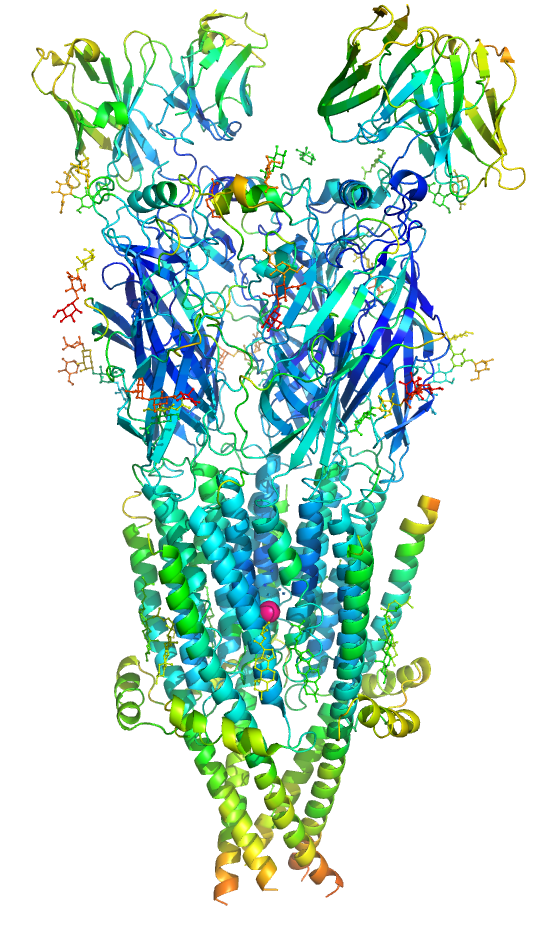
\includegraphics[width=0.3\textwidth]{00_images/6pv7_side_a.png}
%     \caption{Caption}
%     \label{fig:my_label}
% \end{figure}

\vfill
\bigskip
\textbf{Sources}
\begin{enumerate}
    \itemsep0em 
    \item Zhang, Zhi-Ming, et al. "Functional food development: Insights from TRP channels." Journal of Functional Foods 56 (2019) 384-394.
    \item Tombola, F.; Pathak, M. M. and Isacoff, E. Y. How Does Voltage Open an Ion Channel? Annual Review of Cell and Developmental Biology, Annual Reviews, 22 (2006) 23-52.
    \item Dworakowska, B. and Do\l{}owy, K. Ion channels-related diseases. Acta Biochimica Polonica, 47 (2000) 685-703.
\end{enumerate}

\vfill
\textbf{Abbreviations}

\begin{minipage}[t]{0.35\textwidth}
\begin{itemize}
    \setlength{\itemsep}{1pt}
    \setlength{\parskip}{1pt}
    \setlength{\parsep}{0pt}
    \item tbsp: tablespoon
    \item tsp: teaspoon
\end{itemize}
\end{minipage}
\begin{minipage}[t]{0.30\textwidth}
\begin{itemize}
    \setlength{\itemsep}{1pt}
    \setlength{\parskip}{0pt}
    \setlength{\parsep}{0pt}
    \item kg.: kilogram
    \item g: gram
\end{itemize}
\end{minipage}
\begin{minipage}[t]{0.3\textwidth}
\begin{itemize}
    \setlength{\itemsep}{1pt}
    \setlength{\parskip}{0pt}
    \setlength{\parsep}{0pt}
    \item l.: liter
    \item ml.: milliliter
    \item cm.: centimeter
\end{itemize}
\end{minipage}

\mainmatter

%%%%%%%%%%%%%%%%%%
%%% New Recipe %%%
%%%%%%%%%%%%%%%%%%
\recipe[This recipe is rich in onions, notorious for their pungent aroma. When sliced, the damaged cells release enzymes that help form compounds that can activate the TRPA1 and TRPV1 ion channels in sensory neurons, leading to the tear-inducing experience.]
{\textcolor{HBRS}{Musakhan Roll \scriptsize{(Hebah Fatafta})}}
%\textit{Put your goggles out, we’re chopping LOTS of onions!!}\\

%[9 medium onions, 1,5 kg. chicken, 1/3 cup olive oil, 10 flatbread, 4 heaped tbsp.s sumac, pine nuts, spices (1 tsp. cardamom, 2 tbsp.s allspice, 1 cinnamon stick, 1 tsp. whole black pepper, and 1 tsp. white pepper) ]

\serves{6-8}
\prepTime{30 minutes}
\cookTime{1 hour}
\dishType{\maindish}
\dishOther{\meat}

\begin{step}
1.5 kg. chicken
1 tsp. Cardamom
1 stick Cinnamon
1 tsp. Pepper, black
1 tsp. Pepper, white 
2 tbsp.s Allspice
8 cups Water

\method
\textbf{Prepare Chicken}: Cut the chicken into slices and boil with the bay leaf, cinnamon, cardamom, allspice, white pepper, black peppercorns, and ca. 8 cups of water until cooked.
\end{step}

\begin{step}
9 medium Onions
$\frac{1}{3}$ cup Olive oil
1-2 pinches Salt, to taste

\method
\textbf{Cook Onions}: slice onions and cook in olive oil on medium heat until caramelized, adding $\frac{1}{2}$ tsp. salt to speed up cooking.
\end{step}

\begin{step}
4 tbsp.s Sumac
$\frac{1}{4}$ cup Pine nuts

\method
\textbf{Combine}: Mix the cooked chicken with the onions, sumac, and pine nuts.
\end{step}

\begin{step}
10 pieces flatbread

\method
\textbf{Assemble Rolls}: Cut the flatbread in half, add the chicken mixture, tuck in the sides and roll tightly.

\textbf{Bake}: Preheat oven to 350$^o$F (180$^o$C), grease baking pan, place rolls, brush with olive oil and bake for 15-20 minutes until golden.

\textbf{Garnish and Serve}: Add sumac and pine nuts, if desired, and serve warm.
\end{step}

\showpic{0.45}{00_images/musakhan_roll.jpeg}{Image source: https://falasteenifoodie.com/msakhan-rolls}


%%%%%%%%%%%%%%%%%%
%%% New Recipe %%%
%%%%%%%%%%%%%%%%%%
\recipe[This simple satisfying recipe is an example of the interplay between taste receptors, signaling pathways and ion channels that shapes flavor perception.
%My research focuses on the physiological properties of the epithelial sodium channel (ENaC), a key player in sodium transport in our bodies.
%And this recipe highlights the broader context in which ENaC operates.
%In this recipe, the interplay between the sweetness of the onions and potatoes, the umami of the chicken, the saltiness of the rice and broth, and the acidity of the lemon juice creates a harmonious balance that enhances the overall taste experience and demonstrates the complex interplay of factors that contribute to our overall taste experience.
The onions and potatoes sweetness is primarily perceived through the T1R2/T1R3 receptor, while the chicken's umami is detected through the metabotropic glutamate receptor 1 (mGluR1). The balancing acidity of the lemon juice is sensed by sour taste ion-channel receptors (OTOP1). Last but not least, the saltiness of the rice and broth is sensed by the epithelial sodium channel ion channel, which is involved in sodium sensing in taste buds. The interaction between these different taste pathways contributes to the dish's overall flavor profile, highlighting the intricate mechanisms involved in taste perception.]
{\textcolor{HBRS}{Chicken, Rice and Potatoes\\ \textit{A Simple Symphony} \scriptsize{(Sarah Shoushrah})}}

\serves{4}
\prepTime{30 minutes}
\cookTime{1.5 -- 2 hours}
\dishType{\maindish}
\dishOther{\meat}

\begin{step}
2 pieces Chicken thighs, with skin, bones
1 large Onion, peeled and sliced
3 medium Potatoes, peeled and sliced
1 liter Water 
1 dried Bay leaf
2 pods Cardamom
2 pieces Cloves
1-2 pinches Salt and pepper, to taste

\method
\textbf{Prepare the broth}: Place chicken thighs in a pot and cover with water. Bring to a boil until foam forms. Remove chicken, rinse, and return to a cleaned pot. Add onion, potatoes, bay leaf, cardamom, cloves, salt, and pepper. Cover with water and simmer for 1.5-2 hours, or until chicken and potatoes are tender.
\end{step}

\begin{step}
2 cups Basmati rice, washed once
3 cups Water
1 tbsp. Oil or butter
1-2 pinches Salt, to taste

\method
\textbf{Cook the Rice}: Heat oil or butter in a pot. Add washed rice and toast for a few minutes. Stir in salt and water. Bring to a boil, cover, reduce to low medium heat, and simmer for 15-20 minutes, or until rice is tender.

\textbf{Assemble the Dish}: Serve cooked rice with chicken and potatoes. Pour broth over the dish.

\textbf{Recommended}: Squeeze lemon juice over the dish for added flavor.

\textbf{Garnish and Serve}: Serve warm with vanilla or cinnamon ice cream.
\end{step}

%\showpic{0.5}{00_images/01_Mmm..._Apple_Crisp_with_Whipped_Cream.jpeg}{Apple Crisp. Image source: https://upload.wikimedia.org/wikipedia/commons}


%%%%%%%%%%%%%%%%%%
%%% New Recipe %%%
%%%%%%%%%%%%%%%%%%
\recipe[This recipe brings together a variety of ingredients, each offering rich flavors. Ingredients like turmeric, ginger, cinnamon and chili are known to modulate the TRP ion channels, which are located in sensory neurons.]
{\textcolor{HBRS}{Indian Masala Mix Vegetable \scriptsize{(Simran Madaan})}}

% The “crumble” can also be used as a substitute for a pie crust.
% \bigskip

\serves{4}
\prepTime{15 minutes}
\cookTime{30 minutes}
\dishType{\maindish}
\dishOther{\vegan}

\begin{step}
1 whole Onion, diced
1 whole Capsicum (pepper), chopped
2 whole Potatoes, chopped
2-3 cups Cauliflower, chopped
2.5 cm. Ginger, finely diced 
2 cloves Garlic, finely diced 

\method
\textbf{Prepare}: Dice the onion and chop the potato, capsicum and cauliflower into bite-sized pieces. Dice or chop two cloves of garlic and a small piece of fresh ginger for a burst of flavor.
\end{step}

\begin{step}
2 tsp. Mustard Oil

\method
\textbf{Heat and Combine}: In a medium-sized pan, heat the mustard oil until it shimmers, releasing its rich and nutty aroma. Add the diced garlic and ginger, allowing them to sizzle and infuse the oil for about a minute.

\textbf{Sauté}: Toss in the diced onion and sauté until a beautiful golden color.
\end{step}

\begin{step}
$\frac{3}{4}$ tsp. Turmeric
$\frac{1}{2}$ tsp. Garam Masala
1-2 pinches Cinnamon 
1-2 pinches Red chili powder 
1-2 pinches Salt and pepper

\method
\textbf{Spice}: Bring the dish to life with spices. Add the earthy turmeric, a pinch of red chili powder (or smoky paprika), cinnamon and the ``Garam Masala''. Season with salt and freshly ground black pepper to taste.

\textbf{Deepen the Spices}: Let the spices bloom and deepen for a few minutes. Then, add the chopped vegetables and stir well, ensuring that they are coated with the spice mixture.
\end{step}

\begin{step}
1 cup Water
\method
\textbf{Simmer}: Add water and vegetables and simmer gently over medium heat for 10-15 minutes until the potatoes are tender. Add some water as needed to keep everything moist and prevent sticking.
\end{step}

\vspace{-0.6cm}
\showpic{0.30}{00_images/1024px-Aloo_gobi_cauliflower_and_potato_3170159574.jpeg}{}
\vspace{-0.5cm}
\textit{\tiny Image source: https://upload.wikimedia.org/wikipedia/commons}
% Source: https://www.chilipeppermadness.com/recipes/aloo-gobi

%%%%%%%%%%%%%%%%%%
%%% New Recipe %%%
%%%%%%%%%%%%%%%%%%
\recipe[Some cellular ion channels in your body respond to cinnamon. An example of this are the transient receptor potential (TRP) channels. For example, cinnamon includes the small molecule linalool, which is known to interact with the cold-activated cation channel TRPM8.]
{\textcolor{HBRS}{Apple Crisp \scriptsize{(Karl N. Kirschner})}}

\textit{The “crumble” can also be used as a substitute for a pie crust.}
\bigskip

\serves{4}
\prepTime{15 minutes}
\cookTime{45 minutes}
\dishType{\dessert}
\dishOther{\vegetarian}

\begin{step}
5 cups Apples, sliced

\method
\textbf{Apples}: Slice and arrange the applies in a buttered pie or baking dish.
\end{step}

\begin{step}
1 cup Brown sugar
$\frac{3}{4}$ cup Flour, all-purpose
1 tsp. Cinnamon
$\frac{3}{4}$ cup Rolled oats
$\frac{1}{2}$ cup Butter, melted

\method
\textbf{Crumble}: Mix the brown sugar, flour, oats and cinnamon together in its own bowl. Then add the butter and mix again.

\textbf{Combine}: Pour the crumble over the apples so that they are covered well.

\textbf{Bake}: Preheat oven to 175$^o$C. Bake for 45-50 minutes until the crumble's top is golden brown.

\textbf{Garnish and Serve}: Serve warm with vanilla or cinnamon ice cream.
\end{step}
\showpic{0.5}{00_images/01_Mmm_Apple_Crisp_with_Whipped_Cream.jpeg}{}
\textit{Image source: https://upload.wikimedia.org/wikipedia/commons}


%%%%%%%%%%%%%%%%%%
%%% New Recipe %%%
%%%%%%%%%%%%%%%%%%
\recipe[Choline and thiamine are essential for human health. Choline is a precursor to the neurotransmitter acetylcholine, while the thiamine plays a key role in the conversion of pyruvate to acetyl-coA. Both choline and thiamine are transported by  organic cation transporters (OCTs). Spinach contains both choline and, albeit to a lesser degree, thiamine; therefore I thought it would be nice to teach you how to make my mom’s spinach börek.]
{\textcolor{HBRS}{Börek with spinach filling \scriptsize{(Yasemin Aylin Kempf})}}

% \bigskip

\serves{2}
\prepTime{40 minutes}
\cookTime{30 minutes}
\dishType{\maindish}
\dishOther{\vegetarian}

\begin{step}
2 cups Yogurt
2 raw Eggs
$\frac{1}{2}$ cup Oil, plant based
% Some amount Filo dough
% 1-2 pinches spices (sesame seeds, cumin, salt, pepper)
% 1 block of sheep milk cheese (optional)

\method
\textbf{Prepare filling, part 1}: Combine the yogurt with the egg and oil.
\end{step}

\begin{step}
% Some amount Filo dough
500 g. Spinach
2 medium Onions
Few pinches Salt and pepper

\method
\textbf{Prepare the filling, part 2}: Chop spinach and onions and cook them with salt and pepper. Cool afterwards.
\end{step}

\begin{step}
Good amount Filo dough
1 block Sheep cheese, optional

\method
\textbf{Arrange layers}: Cover each layer of the filo dough with the yogurt/egg mixture and add the spinach. Optional: add crumbled sheep milk cheese.
\end{step}

\begin{step}
1-2 pinches Sesame seeds and cumin spices

\method
\textbf{Garnish}: When you are about to run out of the mixture cover the last layer with it and add sesame seeds and cumin on top.

\textbf{Bake}: Preheat oven to 180℃ and add parchment paper. Afterwards bake for 30 minutes until golden (Check occasionally).

\textbf{Serve}: Wait till cooled and then serve.
\end{step}

% %\showpic{0.5}{00_images/lassi_julie_hartbeck.jpg}{Lassi. Image source: https://www.thespruceeats.com/mint-lassi-2216233}

%%%%%%%%%%%%%%%%%%
%%% New Recipe %%%
%%%%%%%%%%%%%%%%%%

\recipe[Menthol is present in different species of mint and activates the ion channel TRPM8. TRPM8 is present in sensory neurons and mediates the sensation of cold. So if you consume mint, menthol stimulates TRPM8, and thereby making your brain believe that something cold or fresh was consumed. That is why a Mint Lassi is a refreshing drink.]
{\textcolor{HBRS}{Mint Lassi \scriptsize{(Avinash Gupta})}}

\textit{No preparation needed, buy ingredients from the supermarket.}
\bigskip

\serves{2}
\prepTime{0 minutes}
\cookTime{2.1 minutes}
\dishType{\drink}
\dishOther{\vegetarian}

\begin{step}
2-3 leaves Mint
2 cups Yogurt (unflavored)
1-2 pinches Pepper
1-2 pinches Salt
2 tbsp. Sugar

\method
\textbf{Cooking process}: Grind or mix the ingredients together in a food processor. Garnish with a mint leaf. If you want to serve it chilled, add ice cubes as desired.

\end{step}
\showpic{0.5}{00_images/1024px-Lassi_5598021969.jpeg}{}
\textit{Image source: https://upload.wikimedia.org/wikipedia/commons}


%%%%%%%%%%%%%%%%%%
%%% New Recipe %%%
%%%%%%%%%%%%%%%%%%
\recipe
[This recipe contains salty potatoes and tasty garlic. Our lab discovered that garlic contains compounds that can inhibit ENaC -- at least in vitro. The Mojo sauce contains chili peppers, which have capsaicin, a TRPV1 ion channel activator that mediates the sensation of heat.]
{\textcolor{HBRS}{Papas arrugadas con mojo rojo – a hot and salty Canary Islands recipe  \scriptsize{(Mike Althaus})}}

\serves{2}
\prepTime{30 minutes}
\cookTime{30 minutes}
\dishType{\maindish}
\dishOther{\meat}

\begin{step}
6 cloves Garlic (peeled)
1 tbsp. Pepper powder
1 tbsp. Caraway seeds
1 tbsp. Dried oregano
1 pinch Chili flakes (to taste)
1 tsp. Sea salt
1-3 pieces Pickled roasted red peppers in vinegar (e.g. “Roter Paprika geröstet” by Dittmann)
1-2 tbsp. Whole unpeeled almonds
Large amount Olive oil

% \textbf{For the Papas arrugadas}:

\method
\textbf{Prepare the Mojo Rojo Sauce}: Add garlic, all herbs, chili and salt to a tall measuring jug. Cover with half of the pickled red peppers. You can include a bit of the vinegar, but it shouldn't be too much. Add the almonds and cover with the remaining pickled red bell pepper. Add olive oil until the ingredients are almost covered. Homogenize with a kitchen blender. If there is too much oil, the sauce will be too dilute - thus, start with a small volume and add more later if necessary. Place the sauce in jars and store in the fridge for a few weeks.
\end{step}

\begin{step}
A few Small unpeeled potatoes 
1 l. Water
Scary amount Sea salt

\method
\textbf{Papas arrugadas}: Cook the unpeeled potatoes for 20-30 min. in water containing sea salt. A scary amount of salt must be added, until the potatoes are floating in the water (mimicing sea water)! After boiling, the potatoes will become wrinkly (“arrugada”). Discard the water and let the potatoes dry in the hot pot. A salt crust will form around the potatoes.

\textbf{Assemble the dish}: Serve the potatoes with the sauce and enjoy!
\end{step}
\vspace{-0.6cm}
\showpic{0.15}{00_images/Foto-Mike.jpeg}


%%%%%%%%%%%%%%%%%%
%%% New Recipe %%%
%%%%%%%%%%%%%%%%%%
\recipe
[Chicken breast is a rich source of actin, a key protein in the actomyosin complex, which is important for cell and muscle movement. Preparing the chicken in this dish involves the chemical reactions of proteins -- such as the Maillard reaction during searing, which enhances flavour through the complex interaction of amino acids and reducing sugars.]
{\textcolor{HBRS}{Gong Bao Chicken \scriptsize{(Julia Weder})}}

% \bigskip

\serves{3}
\prepTime{45 minutes}
\cookTime{15 minutes}
\dishType{\maindish}
\dishOther{\meat}

\begin{step}
400 g. Chicken strips
Large amount Oil
1 tbsp. Flour
1-2 pinches Salt

\method
\textbf{Prepare}: Firstly, generously cover the wok's base with oil and heat to the highest level. Dust the sliced meat all over with flour.

\textbf{Sear} Sear the floured meat in the wok and then season it with salt. Remove the meat.
\end{step}

\begin{step}
50-75 g. Peanuts unsalted and shelled
1 medium Onion diced
2 cloves Garlic
1 bunch Spring onions
2-4 medium Chilli peppers
20 grains Szechuan pepper, crushed
25 g. Cane sugar

\method
\textbf{Fry} Add a little oil if necessary and lightly fry the chopped peanuts. Remove the peanuts and fry the onions. Then, add the chopped garlic and fry it. Cut the spring onions and chilli peppers into strips and add.

\textbf{Caramelize} Sprinkle sugar over and allow the mixture to caramelise.
\end{step}

\begin{step}
1 packet Mie noodles
50 ml. White wine,  or a dash of naturally cloudy apple juice and a dash of lemon juice
1 tbsp. Vinegar
20 ml. Ketjap manis (sweet soy sauce)
2 g. Ginger chopped

\method
\textbf{Noodles} In the meantime, prepare the mie noodles according to the packet instructions.

\textbf{Combine} Add the meat and peanuts again. Deglaze with apple juice and lemon, boil, and add the vinegar—finally, season with soy sauce, ginger and pepper, season to taste and add the noodles. To get it saucy, double the amount of ketjap manis and white wine or apple and lemon juice, depending on how you like it.
\end{step}

%  \showpic{0.5}{00_images/}

%%% From Karen
%%%%%%%%%%%%%%%%%%
%%% New Recipe %%%
%%%%%%%%%%%%%%%%%%
\recipe
[A popular beverage in Mexican is the Margarita. The epithelial sodium channel (ENaC) is essential for sodium homeostasis and the maintenance of the body's blood pressure. It is also expressed in the taste buds, so whenever you eat or drink something salty, ENaC is the channel that enables you taste it. This recipe also contains lime, which stimulates the proton channel OTOP1, a sour receptor in our taste buds. By adding mint, the sensory neurons in your oral cavity will be stimulated by the ion channel TRPM8.]
{\textcolor{HBRS}{Limonada Mineral or Margarita \scriptsize{(Karen Luján})}}

\serves{3}
\prepTime{3 minutes}
\cookTime{5 minutes}
\dishType{\drink}
\dishOther{\vegan}

\begin{step}
2 whole Limes (juice)
1-5 pinches Salt

\method
\textbf{Prepare Glass} Decorate the glass by slicing a lime and rubbing a wedge on the glass rim. Gently, dip the glass's wet rim into the salt, turning it a little so the salt sticks all around the edge.
\end{step}

\begin{step}
1 shot Tequila (optional)

\method
\textbf{Margarita Option} If you are making a margarita, add the tequila shot to the glass now.
\end{step}

\begin{step}
1 glass Sparkling water
3 tbsp. Sugar
1 small handful mint leaves

\method
\textbf{Combine} Fill the decorated glass with ice and top it with the sparkling water, add the sugar and mix until dissolved. Then add the lime juice and mix.

\textbf{Finish Boldly} If you´re feeling bold, add the mint leaves and enjoy!
\end{step}

\showpic{0.45}{00_images/photo-Karen_crop.jpeg}

\end{document}